\documentclass[11pt,a4paper]{article}

\usepackage[utf8]{inputenc}
\usepackage[T1]{fontenc}
\usepackage{lmodern}
\usepackage{microtype}
\usepackage[margin=2.6cm]{geometry}
\usepackage{amsmath,amssymb,amsthm,mathtools}
\usepackage{booktabs}
\usepackage{enumitem}
\usepackage{xcolor}
\usepackage{tikz}
\usetikzlibrary{positioning,arrows.meta,fit}
\usepackage{algorithm}
\usepackage[noend]{algpseudocode}
\usepackage{tcolorbox}
\usepackage[colorlinks=true,linkcolor=blue!50!black,citecolor=blue!50!black,urlcolor=blue!50!black]{hyperref}
\usepackage[capitalise,noabbrev]{cleveref}

\setlength{\emergencystretch}{3em}

\newtheorem{theorem}{Theorem}[section]
\newtheorem{lemma}[theorem]{Lemma}
\newtheorem{corollary}[theorem]{Corollary}
\theoremstyle{definition}
\newtheorem{definition}[theorem]{Definition}
\newtheorem{example}[theorem]{Example}
\theoremstyle{remark}
\newtheorem{remark}[theorem]{Remark}

\newcommand{\code}[1]{\texttt{\small #1}}
\newcommand{\lean}[2]{\code{#1}\,(\code{#2})}
\newcommand{\Sec}{\mathrm{Sec}}
\newcommand{\Dist}{\mathrm{Dist}}
\newcommand{\F}{\mathbb{F}_2}
\newcommand{\cellof}[2]{\langle #1 \mathbin{:} #2\rangle}
\newcommand{\Stab}{\mathrm{Stab}}
\newcommand{\Aut}{\mathrm{Aut}}

\newtcolorbox{intuition}{colback=blue!3,colframe=blue!40!black,boxrule=0.4pt,arc=1pt,left=6pt,right=6pt,top=4pt,bottom=4pt}

\title{Symmetric Cell Search for Probing Security\\[0.3em]
\large How the verifier works, from the netlist to the verdict}
\author{Working notes for the \code{engine-speed} branch}
\date{29 October 2026}

\begin{document}
\maketitle

\begin{abstract}
These notes describe, from start to end, the algorithm that the Lean tool uses to decide
$d$-probing security of a masked Boolean circuit.  A rewrite engine certifies single probe
sets and returns a \emph{coupling}; the coupling extends a certified probe set into a large
\emph{safe set}; a \emph{cell search} covers the space of all probe sets of size $d$ with
few engine calls by remembering every safe set; and the circuit's \emph{automorphisms} are
used twice --- to start the search from cells that contain one representative of every
orbit of probe sets (\emph{orbital branching}), and to settle a probe set whenever a
symmetric image of a stored safe set already contains it (\emph{dominance detection}).
Every step is stated with its soundness argument and with the Lean functions that
implement it.  Section~\ref{sec:orbital} builds the orbital-branching shape of the starting
cells from scratch.
\end{abstract}

\tableofcontents

%======================================================================
\section{Overview}
%======================================================================

The question is whether a circuit is \emph{$d$-probing secure}: whether every set of at
most $d$ wires, observed together, reveals nothing about the secrets.  There are
$\binom{n}{d}$ such sets for a circuit with $n$ wires --- $1\,873\,200$ for the 4-share
DOM Keccak $\chi$ at $d=3$ --- so no tool can afford to examine them one by one.  The
verifier combines four ideas, each of which removes a different kind of redundancy:

\begin{enumerate}[leftmargin=*,label=\textbf{(\arabic*)}]
\item \textbf{Certify one probe set} with a rewrite engine based on optimistic sampling
  (\cref{sec:engine}).  Besides the verdict, the engine returns the change of random
  variables that proved it --- the coupling.
\item \textbf{Extend} the certified probe set: every wire that the same coupling makes
  secret-free can be observed together with it.  This gives a \emph{safe set}, often of
  dozens of wires, and every subset of it is secure (\cref{sec:extension}).
\item \textbf{Search the probe space in cells}: blocks of probe sets described by a few
  numbers, split along safe sets, with every safe set remembered so that the engine is
  called only on probe sets nothing stored covers (\cref{sec:cells}).
\item \textbf{Use the symmetry of the circuit}: an automorphism maps safe sets to safe
  sets.  It is used to start from cells that contain at least one representative of every
  orbit of probe sets (\cref{sec:orbital}) and to recognise probe sets that are symmetric images of covered ones
  (\cref{sec:dominance}).
\end{enumerate}

\begin{figure}[ht]
\centering
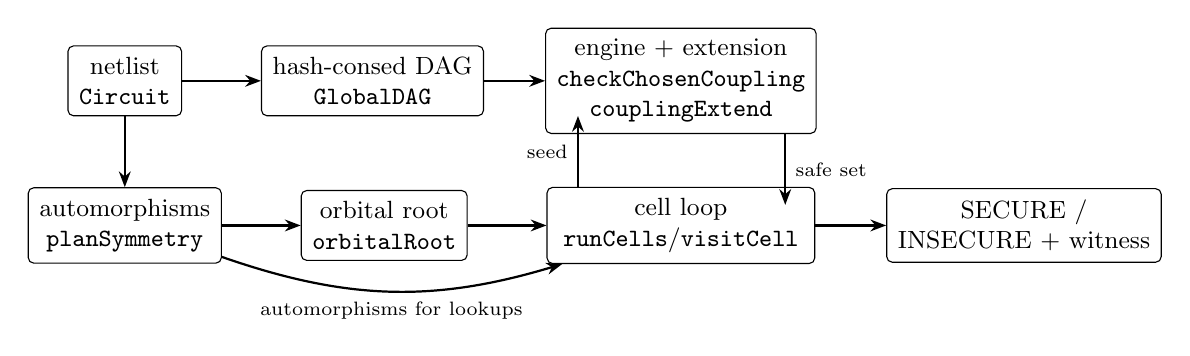
\begin{tikzpicture}[
  box/.style={draw,rounded corners=2pt,align=center,font=\small,minimum height=2.2em,inner sep=4pt},
  arr/.style={-{Stealth[length=2mm]},thick}]
\node[box] (net) {netlist\\ \code{Circuit}};
\node[box,right=1.0cm of net] (dag) {hash-consed DAG\\ \code{GlobalDAG}};
\node[box,below=0.9cm of net] (sym) {automorphisms\\ \code{planSymmetry}};
\node[box,right=1.0cm of sym] (root) {orbital root\\ \code{orbitalRoot}};
\node[box,right=1.0cm of root,minimum width=3.4cm] (loop) {cell loop\\ \code{runCells}/\code{visitCell}};
\node[box] (eng) at (loop |- dag) {engine + extension\\ \code{checkChosenCoupling}\\ \code{couplingExtend}};
\node[box,right=0.9cm of loop] (verdict) {SECURE /\\ INSECURE + witness};
\draw[arr] (net) -- (dag);
\draw[arr] (net) -- (sym);
\draw[arr] (sym) -- (root);
\draw[arr] (root) -- (loop);
\draw[arr] (dag) -- (eng);
\draw[arr] (loop.north west) ++(0.4,0) -- ++(0,0.9) node[midway,left,font=\scriptsize]{seed};
\draw[arr] (eng.south east) ++(-0.4,0) -- ++(0,-0.9) node[midway,right,font=\scriptsize]{safe set};
\draw[arr] (sym) to[bend right=18] node[below,font=\scriptsize]{automorphisms for lookups} (loop);
\draw[arr] (loop) -- (verdict);
\end{tikzpicture}
\caption{The pipeline.  The entry point is \lean{checkDProbingSym}{Symmetry.lean}; the
symmetry-free variant is \lean{checkDProbingCells}{CellSearch.lean}; the older split search
is \lean{checkDProbing}{ProbeClosure.lean}.}
\label{fig:pipeline}
\end{figure}

\paragraph{Where things live.}
\begin{center}\small
\begin{tabular}{@{}lp{9.6cm}@{}}
\toprule
file & contents \\
\midrule
\code{Verif/n-aryDAG.lean} & hash-consed $\F$ DAG; per-node facts (secret dependence, random support, PIT values)\\
\code{Verif/Circuit.lean} & netlist (\code{Circuit}), bridge to the DAG (\code{GlobalDAG})\\
\code{Verif/Engine.lean} & rewrite engine: \code{rewriteComplete}, \code{checkProbeCompleteT}, \code{checkProbeRoots}\\
\code{Verif/Coupling.lean} & extension: \code{couplingExtend}, \code{coneEval}, ANF fallback\\
\code{Verif/ProbeClosure.lean} & split search (\code{checkDProbing}), \code{checkChosenCoupling}, \code{Stats}\\
\code{Verif/CellSearch.lean} & cells, \code{childCells}, \code{SafeStore}, \code{visitCell}, \code{runCells}, audits\\
\code{Verif/Automorphism.lean} & automorphism groups by individualisation--refinement, \code{contractAssoc}\\
\code{Verif/Symmetry.lean} & groups $\to$ wire tables, orbital root, \code{planSymmetry}, \code{checkDProbingSym}\\
\code{Main.lean} & gadget suite, \code{check}, \code{trace}, \code{golden}, \code{bench}\\
\bottomrule
\end{tabular}
\end{center}

A complete run on one gadget, step by step, is printed by
\code{lake exe verif trace "DOM AND (3 shares)"}; \cref{sec:example} walks through it.

%======================================================================
\section{The model}\label{sec:model}
%======================================================================

\paragraph{Circuits.}  A circuit has \emph{leaves} of three kinds --- secrets $s$, randoms
$r$ (independent and uniform over $\F$) and publics --- \emph{input shares}, and
\emph{body wires}.  Every input share and every wire is defined by a gate, an XOR or an AND
of earlier wires, shares, leaves or constants.  Input shares encode the secrets: the
standard sharing of a secret $a$ into $n$ shares uses $n-1$ fresh randoms,
$a_i = r_{a,i}$ for $i<n-1$ and $a_{n-1} = a \oplus \bigoplus_i r_{a,i}$.  The body wires
are what an attacker may probe; input shares are not probe targets (\code{Circuit.inputOrder}
versus \code{Circuit.wireOrder}).  Gates are binary, because in the probing model every
gate output is an observable: an $n$-ary sum hides $n-2$ intermediate values.

Each wire $w$ computes a function $[\![w]\!]$ of the leaves.  For a set $P$ of wires,
$[\![P]\!]$ is the tuple of their values, and for fixed secrets and publics its
\emph{distribution} is taken over the uniform randoms.

\begin{definition}[security of a probe set; safe set]
A set $P$ of wires is \emph{secure}, $\Sec(P)$, if the distribution of $[\![P]\!]$ is the
same for all values of the secrets (for every value of the publics).  We call a set of
wires that is secure a \emph{safe set}.  The circuit is \emph{$d$-probing secure} if every
set of at most $d$ body wires is secure.
\end{definition}

\begin{lemma}[subsets]\label{lem:subset}
Every subset of a safe set is safe.
\end{lemma}
\begin{proof}
The distribution of a sub-tuple is a marginal of the distribution of the tuple; if the
latter does not depend on the secrets, neither does the former.
\end{proof}

Assuming $n \ge d$, it therefore suffices to check every set of \emph{exactly} $d$ wires:
smaller sets are subsets of these.  The converse direction fails, and this matters later.

\begin{remark}[unions are not safe]\label{rem:union}
Two safe sets need not have a safe union.  With a secret $s$ and a random $r$, the wire
$r$ alone and the wire $s\oplus r$ alone are each uniform, hence safe, but together they
reveal $s$.  So the search may never conclude that a probe set is secure because it lies in
the union of two safe sets; it must lie inside \emph{one}.
\end{remark}

\paragraph{The DAG.}  The engine works on a hash-consed DAG of $n$-ary, canonically
ordered XOR and AND nodes (\code{n-aryDAG.lean}): building a node flattens nested XORs,
cancels repeated XOR children, and returns the existing node if the same expression was
built before.  Equal expressions are therefore equal node ids.  Each node also stores,
computed once from its children when it is created (\lean{DAG.alloc}{n-aryDAG.lean}):
whether it depends on a secret (\code{secretDep}), the set of randoms it depends on, as a
bitset (\code{rndSupp}), and its values under 64 parallel pseudo-random evaluations
(\code{valR}, \code{valZ}; used by the extension's fast test).

%======================================================================
\section{Certifying one probe set: the rewrite engine}\label{sec:engine}
%======================================================================

The engine (\code{Engine.lean}) decides $\Sec(P)$ for a probe set $P$ syntactically, by
\emph{optimistic sampling}.

\begin{lemma}[optimistic sampling]
If a random $r$ does not occur in an expression $e$, then the map $r \mapsto e\oplus r$
(all other leaves fixed) is a bijection of the randoms that preserves the uniform
distribution.  Hence substituting $e\oplus r$ for $r$ in every observed expression leaves
the joint distribution of the observations unchanged.
\end{lemma}

The engine applies such substitutions until no observed expression mentions a secret; then
$P$ is secure.  It uses two rules (\lean{rewriteComplete}{Engine.lean}):

\begin{itemize}[leftmargin=*]
\item \textbf{Simple rule.}  A random $r$ that occurs exactly once, inside an XOR node
  $x = e\oplus r$, and is not itself observed: after the substitution $r \leftarrow x$, the
  node $x$ becomes the bare random $r$ --- the whole subexpression $e$ disappears.
  (\code{findSimpleRandom}.)
\item \textbf{General rule.}  A random $r$ with an additive occurrence $x = e\oplus r$,
  $r\notin e$, but other occurrences too: substitute $r\leftarrow x$ everywhere; the matched
  occurrence collapses to $r$ and the others absorb $e$, cancelling where they share it.
  (\code{findGeneralRandom}.)
\end{itemize}

When both rules stall, the engine \emph{factors} ($a\cdot b \oplus a\cdot c \to
a\cdot(b\oplus c)$, \lean{DAG.factor}{n-aryDAG.lean}) to expose randoms buried in products,
and retries.  This is what certifies, for example, the quadratic S-box $Q^4_{12}$, which a
witness replay without factoring rejects.  The engine is sound but incomplete: failure means
``could not prove it'', and the search reports the failed probe set as a counterexample.

\paragraph{The coupling.}  The sequence of substitutions $T = (r_1\leftarrow x_1),\dots,
(r_k\leftarrow x_k)$ is the \emph{coupling} that certified $P$.  It is returned by
\lean{checkProbeCompleteT}{Engine.lean} and consumed by the extension.  (A faster,
reference-counted variant of the simple rule, \code{checkProbeRoots}, is used only by the
split search for verdicts without a coupling.)

%======================================================================
\section{From one probe set to a safe set: the extension}\label{sec:extension}
%======================================================================

\begin{theorem}[coupling extension]\label{thm:extension}
Let $T$ be a coupling under which every expression of the probe set $P$ is secret-free.
Let $S$ be the set of all wires $w$ such that $w\circ T$ --- the expression of $w$ after
the substitutions of $T$ --- is secret-free.  Then $S\supseteq P$ and $S$ is a safe set.
\end{theorem}
\begin{proof}
$T$ is a composition of distribution-preserving bijections of the randoms, so the joint
distribution of $[\![S]\!]$ equals that of the tuple of expressions $(w\circ T)_{w\in S}$.
Each of them is a function of the randoms (and publics) only, so the tuple is too, and its
distribution does not depend on the secrets.
\end{proof}

The point is that \emph{one} coupling serves all wires of $S$ at once, which is why they
are safe \emph{jointly}, not only one by one.  The implementation
(\lean{couplingExtend}{Coupling.lean}) decides membership exactly, but avoids most of the
work:
\begin{itemize}[leftmargin=*]
\item A wire whose random support contains none of the substituted randoms is
  \emph{untouched}: $w\circ T = w$, and its stored secret-dependence bit decides.
\item For a touched wire, a fast rejection test evaluates $w\circ T$ on 64 random
  assignments twice --- secrets random, secrets zero --- re-evaluating only the part of the
  DAG that depends on the substituted randoms (\code{coneEval}).  Any difference proves
  secret dependence.
\item Survivors are accepted only by an exact test: the substituted expression is
  syntactically secret-free, or its algebraic normal form is (\code{anfSecretFreeM}).
\end{itemize}
The chosen probe set is always included, which is what guarantees progress in the search.
Since the 2026-10-28 changes an extension costs 20--40\,$\mu$s on the large gadgets
(the \code{engine-bench} files in \code{lean\_ffi/verif/results/}).

%======================================================================
\section{Covering the probe space: the cell search}\label{sec:cells}
%======================================================================

\subsection{Cells}

\begin{definition}[cell]
A \emph{cell} is a list of pairs $\cellof{c_1}{P_1}\times\dots\times\cellof{c_m}{P_m}$ of
pairwise disjoint wire sets $P_i$ and counts $c_i$.  It stands for the set of probe sets
obtained by choosing $c_i$ wires from each $P_i$; it contains
$\prod_i\binom{|P_i|}{c_i}$ probe sets (\lean{probeCount}{CellSearch.lean}).  Its
\emph{seed} is the probe set made of the first $c_i$ wires of each $P_i$.
\end{definition}

The \emph{root cell} $\cellof{d}{W}$ contains every probe set of size $d$.  A cell is a
compact description of a large, structured block of probe sets: the root cell of Keccak
$\chi$ with 4 shares is one pair of numbers describing $1\,873\,200$ probe sets.

\subsection{Splitting a cell along a safe set}

\begin{lemma}[split]\label{lem:split}
Let $C = \prod_i \cellof{c_i}{P_i}$ be a cell and $S$ a set of wires.  Write
$P_i^{\mathrm{in}} = P_i\cap S$ and $P_i^{\mathrm{out}} = P_i\setminus S$.  Then $C$ is the
disjoint union, over all choices $0\le j_i\le c_i$, of the cells
\[ \textstyle\prod_i \cellof{j_i}{P_i^{\mathrm{in}}}\times\cellof{c_i-j_i}{P_i^{\mathrm{out}}}. \]
The member with $j_i = c_i$ for all $i$ consists of probe sets contained in $S$.
\end{lemma}
\begin{proof}
A probe set of $C$ picks $c_i$ wires from each $P_i$; let $j_i$ be how many of them lie
in $S$.  This determines the member uniquely.  For a single part this is Vandermonde's
identity $\binom{|P|}{c} = \sum_j \binom{|P\cap S|}{j}\binom{|P\setminus S|}{c-j}$.
\end{proof}

If $S$ is safe, the all-in member is settled by \cref{lem:subset} and is dropped; the other
members are the \emph{child cells} (\lean{childCells}{CellSearch.lean}).

\subsection{Remembering safe sets}

Every safe set the search obtains is stored (\code{SafeStore}).  For every wire the store
keeps a bitset over the stored sets that contain it, so ``which stored sets contain all of
the wires $O$?'' is the AND of $|O|$ bitsets (\lean{SafeStore.find}{CellSearch.lean}).
Each stored set is also kept as a wire bitset, for choosing which one to split along.
Two design choices distinguish this search from the classic split search of maskVerif and
of \code{ProbeClosure.lean}:
\begin{itemize}[leftmargin=*]
\item every certified probe set is extended over \emph{all} wires of the circuit, not only
  the wires of the current cell, and the result is kept for the rest of the run;
\item there is no ``union attempt'' (asking the engine to certify all wires of a cell at
  once, which rarely succeeds and costs a large engine call).
\end{itemize}

\subsection{Visiting a cell}

\begin{algorithm}[ht]
\caption{One cell visit (\lean{visitCell}{CellSearch.lean})}\label{alg:visit}
\begin{algorithmic}[1]
\Require cell $C$, store $\mathcal S$ of safe sets, automorphisms $H$ (possibly empty)
\If{some $S\in\mathcal S$ contains every wire of $C$} \Return no children \Comment{skip}
\EndIf
\State $p\gets$ seed of $C$
\If{some $S\in\mathcal S$ contains $p$}
  \State \Return $\mathrm{split}(C, S^\ast)$ \Comment{cover; $S^\ast$: the hit covering most of $C$}
\EndIf
\If{some $h\in H$ and $S\in\mathcal S$ have $h^{-1}(p)\subseteq S$} \Comment{\cref{sec:dominance}}
  \State add $h(S)$ to $\mathcal S$; \Return $\mathrm{split}(C, h(S))$
\EndIf
\State run the engine on $p$ \Comment{\code{checkChosenCoupling}}
\If{not certified} \State stop: INSECURE, counterexample $p$ \EndIf
\State $S\gets$ extension of $p$ over all wires \Comment{\code{couplingExtend}}
\State add $S$ to $\mathcal S$; \Return $\mathrm{split}(C,S)$
\end{algorithmic}
\end{algorithm}

The search keeps a stack of cells, starting from the root cell(s), and visits them
depth-first until the stack is empty (\lean{runCells}{CellSearch.lean}).

\begin{theorem}[cell search]\label{thm:cells}
Started from cells that together contain every probe set of size $d$, the search
terminates.  If it reports SECURE, the circuit is $d$-probing secure; if it reports
INSECURE, the reported probe set could not be certified by the engine.
\end{theorem}
\begin{proof}
\emph{Invariant:} every probe set of the starting cells lies in a cell on the stack or
inside a stored safe set.  A skip removes a cell inside a stored set; a split replaces a
cell by its children and a set that is stored (\cref{lem:split}).  Stored sets are safe:
they come from \cref{thm:extension} or are automorphic images of safe sets
(\cref{thm:transport}).  When the stack is empty every starting probe set is inside a safe
set, hence secure (\cref{lem:subset}); \cref{thm:root} extends this to all probe sets when
the starting cells are the orbital root.
\emph{Termination:} the seed always lies in the set the cell is split along (the engine's
extension contains the seed; a cover contains it by construction), so the dropped all-in
member is non-empty and every child has strictly fewer probe sets than its parent.
\end{proof}

\begin{intuition}
Why cells and not probe sets?  A safe set $S$ of 30 wires settles $\binom{30}{3}=4060$
probe sets of size 3, but they are scattered through any list of probe sets.  In the cell
picture they are exactly one member of a split, removed in one operation; the other members
are described by a handful of numbers each.  The search never lists the probe sets it
settles.
\end{intuition}

Without symmetry ($H=\emptyset$, root $\cellof{d}{W}$) this is
\lean{checkDProbingCells}{CellSearch.lean}.  On the 41-entry suite it is 15 times faster than
the split search (217\,ms against 3\,381\,ms), but Keccak $\chi$ with 4 shares still needs
$14\,706$ engine calls and two seconds.  Symmetry removes most of these.

%======================================================================
\section{Symmetry}\label{sec:symmetry}
%======================================================================

\subsection{Automorphisms and why they preserve safety}

\begin{definition}[automorphism]
A \emph{leaf relabelling} $\alpha$ is a bijection of the leaves that maps secrets to
secrets, randoms to randoms and publics to publics.  It acts on expressions by renaming
leaves.  It \emph{maps wire $w$ to wire $w'$} if relabelling the expression of $w$ gives
exactly the expression of $w'$; where no wire computes the relabelled expression,
$\alpha$ is \emph{not valid} on $w$.  An \emph{automorphism} is such an $\alpha$ together
with its (partial, injective) action on the wires.
\end{definition}

\begin{theorem}[transport; memo Theorem 1]\label{thm:transport}
If $\alpha$ is valid on every wire of $P$, then $\Sec(P) \iff \Sec(\alpha(P))$.
In particular the image of a safe set under an automorphism is a safe set (restricted to
the wires on which it is valid).
\end{theorem}
\begin{proof}[Proof sketch]
The values of $\alpha(P)$ in an environment are the values of $P$ in the environment
pulled back along $\alpha$.  Pulling back permutes the randoms --- a measure-preserving
bijection --- and permutes the secrets, which only reindexes the quantifier ``for all
values of the secrets''.  So the distribution of $[\![\alpha(P)]\!]$ is independent of the
secrets iff that of $[\![P]\!]$ is.  The full proof is in
\code{.ai/AUTOMORPHISM\_PLAN.md}, \S3.
\end{proof}

\begin{remark}[one direction only]
The engine is sound but not equivariant: it may certify $P$ and fail on $\alpha(P)$ (its
tie-breaking depends on node ids).  A \emph{failure} is therefore never transported; only
safety is.
\end{remark}

\subsection{Where the automorphisms come from}

\lean{symmetriesOf}{Symmetry.lean} computes up to two groups:
\begin{itemize}[leftmargin=*]
\item \textbf{Leaf tier.}  Automorphisms of the circuit graph that permute leaves, found by
  individualisation--refinement on a coloured graph \cite{McKayPiperno} and checked exactly
  before they are accepted (\code{automorphisms} and \code{verifyMap} in
  \code{Automorphism.lean}).
\item \textbf{Share tier.}  Treating input shares as atoms, a permutation of the shares of
  a secret is also a symmetry of the joint distribution, provided the sharing is uniform
  and its randoms are used nowhere else.  These two conditions are checked mechanically
  (\code{checkExchangeable}, \code{checkPrivateEncoding}); the tier is skipped when they
  fail.  It sees more symmetry: the leaf tier cannot move the share that carries the
  secret.
\end{itemize}
Both are computed on the \emph{chain-contracted} netlist (\lean{contractAssoc}{Automorphism.lean}),
which merges $u_0\oplus c_{01}\oplus c_{02}$-style XOR chains into single gates.  The chain
order breaks the share symmetry of DOM-AND completely (its as-built group is trivial), and
the contraction recovers it; on the suite the contracted group always contains the as-built
group.  The contracted circuit only \emph{proposes} symmetries: what is used is each
element's action on the real wires, decided exactly by relabelling every wire's expression
and looking up the resulting node (\lean{nameMap}{Symmetry.lean},
\lean{WireTables.of}{Symmetry.lean}).  Chain intermediates such as $s_{0}m_{0}$ simply
come out as ``not valid'' for many elements.

The generators are closed into a list of group elements (\code{closeGroup}).  A group
larger than a bound $B$ (default $64$, \code{defaultGroupCap}) is replaced by the largest
closed subgroup of order at most $B$ found by adding generators one at a time
(\code{closeIncremental}).  Any subgroup is sound; a smaller one costs less to set up and to
look up through, and prunes less (\cref{sec:measure}).

Each element becomes a \emph{wire table}: an array giving, for each wire, its image, or
``not valid''.  Tables are injective where valid, so inverses exist
(\lean{invertTable}{Symmetry.lean}).

\subsection{Groups, orbits and stabilisers in this setting}

The group $G$ acts on wires and, element by element, on probe sets:
$h(P) = \{h(w) : w\in P\}$ when $h$ is valid on every wire of $P$.  The \emph{orbit} of a
probe set $P$ is the set of all its images.  By \cref{thm:transport}, all members of an orbit
are secure or none is: \textbf{it suffices to establish security for one representative of
every orbit.}  The \emph{stabiliser} of a wire $x$ is the subgroup $\Stab(x) = \{h\in G :
h(x)=x\}$.

Two uses of this fact follow.  The first is local and simple (\cref{sec:dominance}); the
second shapes the whole search (\cref{sec:orbital}).

%======================================================================
\section{Symmetry use 1: dominance before the engine}\label{sec:dominance}
%======================================================================

When no stored safe set contains a cell's seed $p$, the engine would be called.  Before
that, the search asks whether a symmetric image of a stored set contains $p$:

\begin{lemma}[dominance]\label{lem:dominance}
If $h$ is an automorphism, $S$ a stored safe set, and $h^{-1}(p)\subseteq S$ (that is,
$h^{-1}$ is valid on $p$ and maps it into $S$), then $p\subseteq h(S)$ and $h(S)$ is safe.
\end{lemma}
\begin{proof}
Every wire of $p$ is $h$ of a wire of $S$, so lies in $h(S)$; $h(S)$ is safe by
\cref{thm:transport}.
\end{proof}

The search maps $p$ backwards --- $d$ table lookups per automorphism --- and asks the store
as before (\lean{findThroughSymmetry}{CellSearch.lean}).  The image $h(S)$ is then stored
as an ordinary safe set and the cell is split along it, so later lookups find it without
symmetry.  This is the probing-security analogue of symmetry breaking by dominance
detection in constraint programming \cite{FahleSchambergerSellmann,FocacciMilano}: a
subproblem is skipped if a symmetric image of it is dominated by work already done.

Two details matter for speed.  The lookup through symmetry runs only when the
alternative is an engine call, not at every cell.  And mapping the \emph{seed} backwards
(instead of storing every image of every safe set) keeps the store's size independent of
the group order.

%======================================================================
\section{Symmetry use 2: orbital branching for the starting cells}\label{sec:orbital}
%======================================================================

Dominance removes engine calls, but the search still \emph{visits} cells for probe sets
whose symmetric images were already handled.  On Keccak $\chi$ with 4 shares, searching
from the single root cell with dominance lookups visits $60\,478$ cells and takes 430\,ms;
starting from the orbital root it visits $13\,373$ cells and takes 140\,ms.  This section
explains what the orbital root is and why it has its shape.

\subsection{The goal, and why not canonical forms}

We want starting cells that contain \emph{at least one} member of every orbit of probe
sets --- ideally few more.  A textbook approach lists all probe sets and keeps those that
are lexicographically smallest in their orbit (a canonical-form test, as in orderly
generation \cite{McKayIsomorphFree}).  That defeats the purpose here: it lists every probe
set, while the cell search is built to avoid listing any.  We need cells --- large blocks
described by a few numbers --- that are guaranteed to contain a representative of every
orbit.  Orbital branching produces exactly that.

\subsection{One wire}

For $d=1$ the answer is immediate: a probe set is one wire, its orbit is the wire's orbit,
and one wire per orbit suffices.

\subsection{The branching rule}

Now take $d$ arbitrary and one orbit $O$ of wires, with a chosen representative $x\in O$.
Every probe set either meets $O$ or avoids it.

\begin{lemma}[orbital branching]\label{lem:ob}
If a probe set $P$ meets $O$, some $h\in G$ maps $P$ to a probe set containing $x$.
\end{lemma}
\begin{proof}
Pick $y\in P\cap O$; since $y$ and $x$ are in the same orbit, some $h$ has $h(y)=x$, so
$x\in h(P)$.
\end{proof}

So the probe sets that meet $O$ need only be examined \emph{in the form that contains $x$}:
\[
\{P : P\cap O\neq\emptyset\}\ \leadsto\ \{P : x\in P\}, \qquad
\{P : P\cap O=\emptyset\}\ \text{kept as is.}
\]
This is the two-way branching of \emph{orbital branching} in integer programming
\cite{Ostrowski}: on an orbit $O$ of 0/1 variables, branch into ``$x_j = 1$ for one
representative $j\in O$'' and ``$\sum_{i\in O} x_i = 0$''; the other $|O|-1$ branches
``$x_i=1$'' are symmetric copies of the first and are never explored.  Here the variables
are ``wire $w$ is probed'' and $\sum_w x_w = d$.

\subsection{Repeating it over all orbits: the shape of the first level}

Order the orbits of wires $O_1, O_2, \dots, O_k$ and fix a representative $x_i\in O_i$.
Apply the rule to $O_1$: probe sets that meet $O_1$ become ``contains $x_1$''; the rest avoid
$O_1$.  Apply it again, to $O_2$, on the probe sets that avoid $O_1$, and so on.  After the
last orbit nothing is left (a probe set meets some orbit).  The pieces are:
\[
\boxed{\ \cellof{1}{\{x_i\}}\ \times\ \cellof{d-1}{(O_i\setminus\{x_i\})\cup O_{i+1}\cup\dots\cup O_k}\qquad i=1,\dots,k.\ }
\]
This is the shape of the starting cells: \textbf{the $i$-th cell is pinned to the
representative of orbit $i$, and the other $d-1$ wires come from the rest of that orbit and
the later orbits.}  The earlier orbits are missing because a probe set reaching cell $i$
was, by construction, one that avoids $O_1,\dots,O_{i-1}$ --- each probe set is assigned to
the \emph{first} orbit it meets.  (Missing them is not needed for soundness; it is what makes
the cells disjoint, so nothing is examined twice for that reason.)

\begin{example}[two orbits, a rotation]\label{ex:c3}
Six wires $a_0,a_1,a_2,b_0,b_1,b_2$ and the rotation $\rho: a_i\mapsto a_{i+1},\ b_i\mapsto
b_{i+1}$ (indices mod 3), generating a group of order 3.  For $d=2$ there are 15 pairs; no
pair is fixed by $\rho$, so there are $15/3 = 5$ orbits.  The orbits of wires are $A$ and
$B$.  The branching gives
\[
\cellof{1}{\{a_0\}}\times\cellof{1}{\{a_1,a_2,b_0,b_1,b_2\}}\ (5\text{ pairs}),\qquad
\cellof{1}{\{b_0\}}\times\cellof{1}{\{b_1,b_2\}}\ (2\text{ pairs}),
\]
7 pairs instead of 15.  Two orbits are still represented twice: $\{a_0,a_1\}$ and
$\{a_0,a_2\}$ ($\rho^2$ maps the first to the second), and likewise $\{b_0,b_1\}$,
$\{b_0,b_2\}$.  The reason is that a pair with \emph{two} wires in its first orbit can be
rotated to contain $x$ in two ways.  These remaining duplicates are what dominance
(\cref{sec:dominance}) removes when the search reaches them.
\end{example}

\subsection{The remaining wires: stabilisers and recursion}

Inside cell $i$, the wire $x_i$ is fixed.  Every element that fixes $x_i$ --- the stabiliser
$\Stab(x_i)$ --- maps the cell's probe sets to probe sets that still contain $x_i$, so it is
still a symmetry of the sub-problem ``choose the remaining $d-1$ wires from $F_i =
(O_i\setminus\{x_i\})\cup O_{i+1}\cup\dots$''.  So we branch again, inside $F_i$, on the
orbits of $\Stab(x_i)$, with the same rule.  Each level pins one more wire and passes to a
smaller group, until all $d$ wires are pinned or the group becomes trivial; then the
remaining choice is left as a plain block.  This is a stabiliser chain, and the cells are
the leaves of the branching tree (\lean{obranch}{Symmetry.lean}, \lean{pinClass}{Symmetry.lean}).

\begin{example}[a ring, with and without reflections]\label{ex:ring}
Six wires $w_0,\dots,w_5$ on a ring, $d=2$: 15 pairs in 3 orbits (distance 1, 2, 3).
\begin{itemize}[leftmargin=*]
\item Under the rotations $C_6$ there is one orbit of wires; the first level gives
  $\cellof{1}{\{w_0\}}\times\cellof{1}{\{w_1,\dots,w_5\}}$ (5 pairs).  The stabiliser of
  $w_0$ in $C_6$ is trivial, so the recursion stops: 5 pairs for 3 orbits ($\{w_0,w_1\}$ and
  $\{w_0,w_5\}$ are the same orbit).
\item Under the dihedral group $D_6$ (rotations and reflections) the stabiliser of $w_0$
  contains the reflection $w_i\leftrightarrow w_{-i}$.  Its orbits on the remaining wires are
  $\{w_1,w_5\}$, $\{w_2,w_4\}$, $\{w_3\}$, and branching on them gives the three cells
  $\{w_0,w_1\}$, $\{w_0,w_2\}$, $\{w_0,w_3\}$ --- exactly one pair per orbit.
\end{itemize}
The larger the stabilisers, the closer the cells come to one representative per orbit.
\end{example}

Orbits of size one (wires every element fixes) gain nothing from pinning; they are kept
together as one plain part (``\code{fix}'' in \code{pinClass}).

\subsection{Partial symmetry: stable domain and loose wires}

So far every element was valid on every wire.  In real circuits it is not: a chain
intermediate like $s_0m_0 = u_0\oplus c_{01}$ has no image under most share permutations.
\Cref{lem:ob} needs, for a probe set $P$, an element valid on \emph{all} of $P$; and the
recursion composes elements, so validity must survive composition.  The construction
therefore works on the \emph{stable domain} of the current group $K$ inside the current
wire set $F$:
\[ D = \{w\in F : \text{every } h\in K \text{ is valid on } w \text{ and } h(w)\in F\}
\qquad(\code{stableIn}). \]
Because $K$ is a closed group and validity is decided exactly, $D$ is mapped onto itself
by $K$, every composition of elements stays valid on $D$, and the branching of the previous
subsections is applied to $D$.  This is why the group is \emph{listed and closed} rather
than kept as generators: orbits and stabilisers on $D$ are then those of a genuine group
acting by permutations.

The wires of $F\setminus D$ are \emph{loose}.  Probe sets that touch a loose wire are
handled in three steps (\lean{looseClass}{Symmetry.lean}):
\begin{enumerate}[leftmargin=*]
\item look for a subgroup $K_2\le K$ --- the elements mapping some set of loose wires onto
  itself --- whose stable domain is larger and covers some loose wires
  (\code{bestSubgroup}), and branch with $K_2$ on the newly covered wires;
\item a loose wire whose own stabiliser still moves other wires gets its own pinned cell,
  with that stabiliser for the recursion;
\item the remaining loose wires form plain cells: $j$ of them, and $d-j$ wires of $D$.
\end{enumerate}
In DOM-AND with 3 shares the products $u_i,p_{ij}$ and the outputs $s_i$ form the stable
domain of the share group; the masked terms $c_{ij}$ are loose but have a subgroup that
permutes them; the chain intermediates $s_im_0$ are loose with small stabilisers.  The
resulting root is listed in \cref{sec:example}.

\subsection{Branching only where it pays}

Cutting a cell by orbits replaces it by several smaller cells.  If the group is small, the
cut removes few probe sets but fragments the cell, and large cells serve the stored safe sets
better (one safe set removes a whole member of a large cell in one split).  So each branching
step is kept only if it removes at least a quarter of the cell's probe sets; otherwise the
cell is kept whole (in \lean{obranch}{Symmetry.lean}).  For ISW-AND with 5 shares (a group of
order 2) the cut would keep 79\,\% of the probe sets in $15$ cells; the rule keeps the single
root cell, and dominance lookups still catch the symmetric repeats.

\subsection{Correctness}

\begin{theorem}[orbital root]\label{thm:root}
For every probe set $P$ of size $d$ there is a group element valid on $P$ that maps $P$
into a cell of the orbital root.  Consequently, if every probe set of the orbital root is
secure, every probe set is.
\end{theorem}
\begin{proof}[Proof sketch]
By induction along the branching tree.  At a node with group $K$, prefix $\mathit{pre}$
(fixed pointwise by $K$), wire set $F$ and count $c$, let $Q$ be the part of the probe set
still to place.  If the node is kept whole the claim is trivial.  If $Q$ meets the stable
domain $D$ in a non-trivial orbit, let $O_i$ be the first such orbit it meets; an element of
$K$ maps a wire of $Q\cap O_i$ to $x_i$ (\cref{lem:ob}); $K$ preserves each orbit, so the
image still avoids $O_1,\dots,O_{i-1}$ and lies in the $i$-th child; recurse with
$\Stab(x_i)$, composing the elements (valid on $D$).  If $Q\cap D$ lies in fixed wires, the
fixed-part cells contain it.  If $Q$ touches loose wires, the loose-wire cases enumerate all
possibilities, using subgroups of $K$.  Every element used fixes $\mathit{pre}$.  The second
sentence follows from \cref{thm:transport}.
\end{proof}

The implementation checks the first statement by brute force on every gadget whose size
permits it: every probe set must be mapped into a root cell by some listed element
(\lean{rootCheck}{Symmetry.lean}, part of \code{lake exe verif golden}).

\begin{intuition}
Orbital branching and dominance are complementary.  Orbital branching decides, before the
search starts and without looking at any probe set, which blocks need to be searched at
all; it cannot see the duplicates that remain inside the blocks (\cref{ex:c3}).  Dominance
sees exactly those, one seed at a time, but only after the search has reached them.
Measured on Keccak $\chi$ with 4 shares: dominance alone 430\,ms, both 140\,ms.
\end{intuition}

%======================================================================
\section{The complete algorithm}\label{sec:complete}
%======================================================================

\begin{algorithm}[ht]
\caption{Symmetric cell search (\lean{checkDProbingSym}{Symmetry.lean})}\label{alg:full}
\begin{algorithmic}[1]
\Require circuit with body wires $W$, order $d$
\State groups $\gets$ leaf tier and share tier of the chain-contracted netlist, each closed and bounded by $B$
\State $H\gets$ all non-identity elements, as forward and inverse wire tables
\State roots $\gets$ the orbital root of whichever group gives the fewer probe sets
\State stack $\gets$ roots; $\mathcal S\gets\emptyset$
\While{stack not empty}
  \State pop a cell and visit it (\cref{alg:visit}); on INSECURE stop
  \State push its children
\EndWhile
\State \Return SECURE
\end{algorithmic}
\end{algorithm}

\begin{theorem}
\Cref{alg:full} terminates.  If it returns SECURE, the circuit is $d$-probing secure.
\end{theorem}
\begin{proof}
Every probe set of the roots ends inside a stored safe set (\cref{thm:cells}); stored sets
are safe (\cref{thm:extension}, \cref{lem:dominance}); every probe set has an image in the
roots (\cref{thm:root}) and security transports along it (\cref{thm:transport}).
\end{proof}

%======================================================================
\section{Worked example: DOM-AND with 3 shares at order 2}\label{sec:example}
%======================================================================

The gadget has 21 body wires: products $u_i = a_ib_i$ and $p_{ij}=a_ib_j$, masked cross
terms $c_{ij} = p_{ij}\oplus r_{ij}$ (with $c_{ji}$ using the same $r_{ij}$), and outputs
built as chains $s_im_0 = u_i\oplus c_{i\cdot}$, $s_i = s_im_0\oplus c_{i\cdot}$.
There are $\binom{21}{2}=210$ pairs.  The output below is from
\code{lake exe verif trace "DOM AND (3 shares)"}.

\paragraph{Symmetry.}  Leaf tier of order 4; share tier of order $36 = 3!\cdot 3!$ (the
shares of $a$ and the shares of $b$ permuted independently; most elements are valid on only
part of the wires); 35 distinct non-identity automorphisms for the lookups.  A typical element swaps share indices 0 and 1:
$u_0\leftrightarrow u_1$, $p_{01}\leftrightarrow p_{10}$, $c_{02}\leftrightarrow c_{12}$,
$s_0\leftrightarrow s_1$, \dots, and is not valid on $s_2m_0$ (the chain
$u_2\oplus c_{20}$ would become $u_2\oplus c_{21}$, which no wire computes).

\paragraph{Orbital root: 62 of 210 pairs in 9 cells.}
\begin{center}\small
\begin{tabular}{@{}lr@{}}
\toprule
cell & pairs \\
\midrule
$\{u_0,u_1\}$, $\{u_0,p_{01}\}$, $\{u_0,p_{10}\}$, $\{u_0,s_1\}$, $\{u_0,s_0\}$, $\{s_0,s_1\}$ & $6\times 1$\\
$\cellof{1}{\{c_{01}\}}\times\cellof{1}{\{c_{10},c_{02},c_{20},c_{12},c_{21},u_\ast,p_\ast,s_\ast\}}$ & 17\\
$\cellof{1}{\{s_0m_0\}}\times\cellof{1}{\{s_1m_0,u_\ast,p_\ast,c_\ast,s_\ast\}}$ & 19\\
$\cellof{1}{\{s_2m_0\}}\times\cellof{1}{\{\text{all other 20 wires}\}}$ & 20\\
\bottomrule
\end{tabular}
\end{center}
The first six cover the 66 pairs inside the stable domain $\{u_\ast,p_\ast,s_\ast\}$ (the
12 wires on which every element is valid): the branching pinned $u_0$ (orbit of the
products), then pinned the second wire within the orbits of $\Stab(u_0)$; the pair
$\{s_0,s_1\}$ comes from the next orbit, the outputs.  The $c_{ij}$ are loose for the whole
group, but a subgroup permutes them, so every pair containing a masked term is represented by
a pair containing $c_{01}$.  The chain intermediates are the least symmetric: $s_2m_0$ gets
its own pinned cell, whose further cutting does not pay (20 pairs, kept whole); $s_0m_0$
and $s_1m_0$ are exchanged by the group, so pairs with $s_1m_0$ are represented in the
$s_0m_0$ cell.

\paragraph{The search: 28 cell visits, 9 engine calls.}
\begin{center}\small
\begin{tabular}{@{}rp{11.2cm}@{}}
\toprule
step & what happens \\
\midrule
1 & cell $\{u_0,u_1\}$: engine certifies it; extension gives
    $\{u_0,u_1,p_{01},p_{10},c_{01},c_{10},s_0m_0,s_1m_0\}$, stored.\\
2--3 & $\{u_0,p_{01}\}$ and $\{u_0,p_{10}\}$: skipped, inside that set.\\
4 & $\{u_0,s_1\}$: engine; stores $\{u_0,s_1,u_1,p_{01},p_{10}\}$.\\
5 & $\{u_0,s_0\}$: \emph{dominance} --- swapping share indices 0 and 1 maps $\{u_0,s_0\}$ to
    $\{u_1,s_1\}$, inside the set of step 4; the image $\{u_0,u_1,p_{01},p_{10},s_0\}$ is
    stored.  No engine call.\\
6 & $\{s_0,s_1\}$: engine; stores $\{s_0,s_1,u_0,u_1,p_{01},p_{10}\}$.\\
7 & the $c_{01}$ cell (17 pairs): its seed $\{c_{01},c_{10}\}$ is inside the set of step 1;
    split into children.\\
8--14 & the $c_{01}$ children: 3 engine calls, 4 dominance hits.\\
15--21 & the $s_0m_0$ cell: 2 engine calls, 2 dominance hits, 2 covers, 1 skip.\\
22--28 & the $s_2m_0$ cell: 1 engine call, 5 dominance hits, 1 cover.\\
\midrule
total & 9 engine calls, 16 covers (12 of them through symmetry), 3 skips, 21 stored sets.\\
\bottomrule
\end{tabular}
\end{center}
For comparison: without symmetry the same search makes 30 engine calls and 68 cell visits;
the split search makes 84 engine calls (including union attempts); maskVerif checks the 435
pairs of its own, larger observation set.

%======================================================================
\section{How the implementation is checked}\label{sec:checks}
%======================================================================

Every change on the branch must leave the following check unchanged (176 lines):
\begin{center}\code{lake exe verif golden check results/engine-golden\_baseline.txt}\end{center}
It records:
\begin{itemize}[leftmargin=*]
\item for every gadget, the engine's verdict, coupling and extension on 100--300 seeded
  random probe sets, in a node-id-independent form (detects any change in the engine);
\item the end-to-end result of the split search, the cell search and the symmetric search;
\item \textbf{coverage audit}: after a secure run, every probe set of the starting cells lies
  inside a stored safe set (\code{coverageAudit}, \code{coverageAuditCells}) --- checked by
  enumeration, e.g.\ all $1\,873\,200$ triples of Keccak $\chi$ with 4 shares;
\item \textbf{root audit}: every probe set is mapped into a root cell by a listed element
  (\code{rootCheck}); skipped only for the two largest gadgets (budget);
\item the one-pass \code{contractAssoc} against its step-by-step definition
  (\code{golden contract}).
\end{itemize}
The two audits re-check, independently of the search's own bookkeeping, the two facts its
soundness rests on (\cref{thm:cells,thm:root}).  Safety of each stored set itself rests on the
engine and \cref{thm:extension,thm:transport}.

%======================================================================
\section{Measurements}\label{sec:measure}
%======================================================================

All figures are from 28--29 October 2026 on one desktop machine under light background load
($\pm 20\,\%$); details in \code{lean\_ffi/verif/results/}.

\paragraph{What each idea contributes} (milliseconds, in process, setup included):
\begin{center}\small
\begin{tabular}{@{}lrrrr@{}}
\toprule
 & \shortstack{split\\search} & \shortstack{cells,\\no symmetry} & \shortstack{cells +\\dominance only} & \shortstack{full\\(Alg.~\ref{alg:full})}\\
\midrule
41-entry suite (sum) & 3\,381 & 217 & --- & 246\\
DOM Keccak $\chi$, 4 shares, $d=3$ & $>25$\,min$^\ast$ & 1\,981 & 430 & 140\\
DOM-AND, 5 shares, $d=4$ & --- & 119 & 240$^\dagger$ & 90\\
ISW-AND, 5 shares, $d=4$ & 586 & 62 & --- & 71\\
\bottomrule
\end{tabular}\\[2pt]
{\footnotesize $^\ast$ before the engine changes. $^\dagger$ with groups bounded at 600 instead of 64.}
\end{center}

\paragraph{The group bound.}  Groups of order 576 and more (DOM-AND with 4 and 5 shares)
cost more to list, tabulate, branch on and look up through than they save: at bound 600
DOM-AND-5 takes 203\,ms, at 64 it takes 84--90\,ms.  Keccak $\chi$ (orders 10 and 30) is
unaffected at 64 and loses 40\,\% at 24.

\paragraph{Against maskVerif} (one process per gadget, best of 3, each tool's start-up time
subtracted; \code{results/maskverif-comparison\_2026-10-28.md}):
\begin{center}\small
\begin{tabular}{@{}lrr@{}}
\toprule
gadget & maskVerif [ms] & this tool [ms]\\
\midrule
DOM Keccak $\chi$, 4 shares, $d=3$ & 426 & 140\\
DOM-AND, 5 shares, $d=4$ & 371 & 85\\
ISW-AND, 5 shares, $d=4$ & 213 & 66\\
DOM-AND, 4 shares, $d=3$ & 27 & 11\\
DOM Keccak $\chi$, 3 shares, $d=2$ & 18 & 8\\
TI Fides AB1, $d=1$ & 12 & 26\\
33 secure suite entries (sum) & 331 & 156\\
\bottomrule
\end{tabular}
\end{center}
The verdicts agree on all 44 gadgets.  maskVerif \cite{maskVerif} also probes input shares
and randoms (275 against 225 positions on Keccak $\chi$ with 4 shares).

%======================================================================
\section{Limitations and open questions}\label{sec:limits}
%======================================================================

\begin{itemize}[leftmargin=*]
\item \textbf{Fixed parameters.}  The group bound 64 and the ``at least a quarter'' rule were
  measured on this suite only.
\item \textbf{Not one representative per orbit.}  The root leaves duplicates whenever a
  probe set meets its first orbit twice (\cref{ex:c3}) or the stabilisers are small; dominance
  removes them later, at the cost of a lookup.
\item \textbf{Partial symmetry.}  The loose-wire construction is a heuristic choice of
  subgroups; its correctness is checked by \code{rootCheck}, not proved in Lean.
\item \textbf{TI Fides AB1.}  Its couplings relabel the input-encoding randoms, which almost
  every wire depends on, so nearly every candidate needs the slow path of the extension.
\item \textbf{Model.}  Value-based probing only; glitches and transitions are out of scope.
  Symmetry is cheaper to use in this model, because two wires with the same value function are
  interchangeable.
\item \textbf{Proof status.}  \Cref{thm:transport,thm:extension} are argued in the design memo;
  the Lean formalisation on the \code{formally-verified} branch covers the engine and the
  split search, not the cell search or the symmetry.
\end{itemize}

\begin{thebibliography}{9}\small
\bibitem{ISW} Y.~Ishai, A.~Sahai, D.~Wagner.  Private circuits: securing hardware against
  probing attacks.  CRYPTO 2003.
\bibitem{BartheEC15} G.~Barthe, S.~Bela\"{\i}d, F.~Dupressoir, P.-A.~Fouque, B.~Gr\'egoire,
  P.-Y.~Strub.  Verified proofs of higher-order masking.  EUROCRYPT 2015.
\bibitem{maskVerif} G.~Barthe, S.~Bela\"{\i}d, G.~Cassiers, P.-A.~Fouque, B.~Gr\'egoire,
  F.-X.~Standaert.  maskVerif: automated verification of higher-order masking in presence of
  physical defaults.  ESORICS 2019.
\bibitem{Ostrowski} J.~Ostrowski, J.~Linderoth, F.~Rossi, S.~Smriglio.  Orbital branching.
  Mathematical Programming 126(1), 2011.
\bibitem{Margot} F.~Margot.  Pruning by isomorphism in branch-and-cut.  Mathematical
  Programming 94, 2002.
\bibitem{FahleSchambergerSellmann} T.~Fahle, S.~Schamberger, M.~Sellmann.  Symmetry breaking.
  CP 2001.
\bibitem{FocacciMilano} F.~Focacci, M.~Milano.  Global cut framework for removing symmetries.
  CP 2001.
\bibitem{McKayIsomorphFree} B.~D.~McKay.  Isomorph-free exhaustive generation.  Journal of
  Algorithms 26, 1998.
\bibitem{McKayPiperno} B.~D.~McKay, A.~Piperno.  Practical graph isomorphism, II.  Journal of
  Symbolic Computation 60, 2014.
\end{thebibliography}

\end{document}
